\section{Parallel Algorithms}
\label{sec:parallel}

\subsection{Naive Parallel NMF Algorithm} 
\label{sec:naive}

In this section we present a naive parallelization of NMF algorithms, which has previously appeared in the context of a shared-memory parallel platform \cite{Fairbanks2015}. 
Each NLS problem with multiple right-hand sides can be parallelized based on the observation that each right-hand side is independent from the others. 
For example, we can solve several instances of Eq.~\eqref{eqn:single NLS} independently for different $\mathbf{b}$ where $\CC$ is fixed, which implies that we can optimize row blocks of $\WW$ and column blocks of $\HH$ in parallel. 
%\ramki{In this paper  we are using BPP to solve this Non-negative Least Squares (NLS) problem and call the algorithm as Naive Parallel BPP(\NaiveAlg). But the conversation in this section is not limited to \NaiveAlg and with out loss of generality is applicable to any algorithm that follows ANLS Algorithm \ref{alg:anlsnmf} such as Multiplicative Update (MU) and HALS as well.}



\begin{algorithm}[t!]
\caption{$[\WW,\HH] = \text{\NaiveAlg}(\AA,k)$}
\label{alg:naive}
\begin{algorithmic}[1]
\Require $\AA$ is an $m\times n$ matrix distributed both row-wise and column-wise across $p$ processors, $k$ is the approximation rank
\Require Local matrices: $\AA_{i}$ is $m/p\times n$, $\AA^{i}$ is $m\times n/p$, $\WW_i$ is $m/p\times k$, $\HH^i$ is $k\times n/p$
\State $p_i$ initializes $\HH^i$
\While{stopping criteria not satisfied}
	\Statex \quad\; \textbf{/* Compute $\WW$ given $\HH$ */} 
	\State collect $\HH$ on each processor using all-gather
		\label{line:naive:allgatherH}
	%\Statex \quad\; \textbf{/* Use Equation \eqref{eqn:muupdate}, \eqref{eqn:halsupdate} for \MU\ and \HALS\ respectively. ANLS/BPP will implement the SolveBPP function \ref{sec:BPP}.*/} 	
	\State $p_i$ computes $\WW_i \gets$ updateW$(\HH\HH^T,\AA_i\HH^T)$
		\label{line:naive:computeW}
	\Statex \quad\; \textbf{/* Compute $\HH$ given $\WW$ */} 
	\State collect $\WW$ on each processor using all-gather
		\label{line:naive:allgatherW}
	%\Statex \quad\; \textbf{/* Use Equation \eqref{eqn:muupdate},\eqref{eqn:halsupdate} for \MU\ and \HALS\ respectively. ANLS/BPP will implement the SolveBPP function \ref{sec:BPP}.*/} 	
	\State $p_i$ computes $(\HH^i)^T \gets$ updateH$(\WW^T\WW,(\WW^T\AA^i)^T)$
		\label{line:naive:computeH}
\EndWhile
\Ensure $\displaystyle \WW, \HH \approx \Argmin{\M{\tilde W} \geq 0, \M{\tilde H} \geq 0} \|\AA- \M{\tilde W} \M{\tilde H}\|$
\Ensure $\WW$ is an $m\times k$ matrix distributed row-wise across processors, $\HH$ is a $k\times n$ matrix distributed column-wise across processors
\end{algorithmic}
\end{algorithm}

\begin{figure}[t!]
\centering
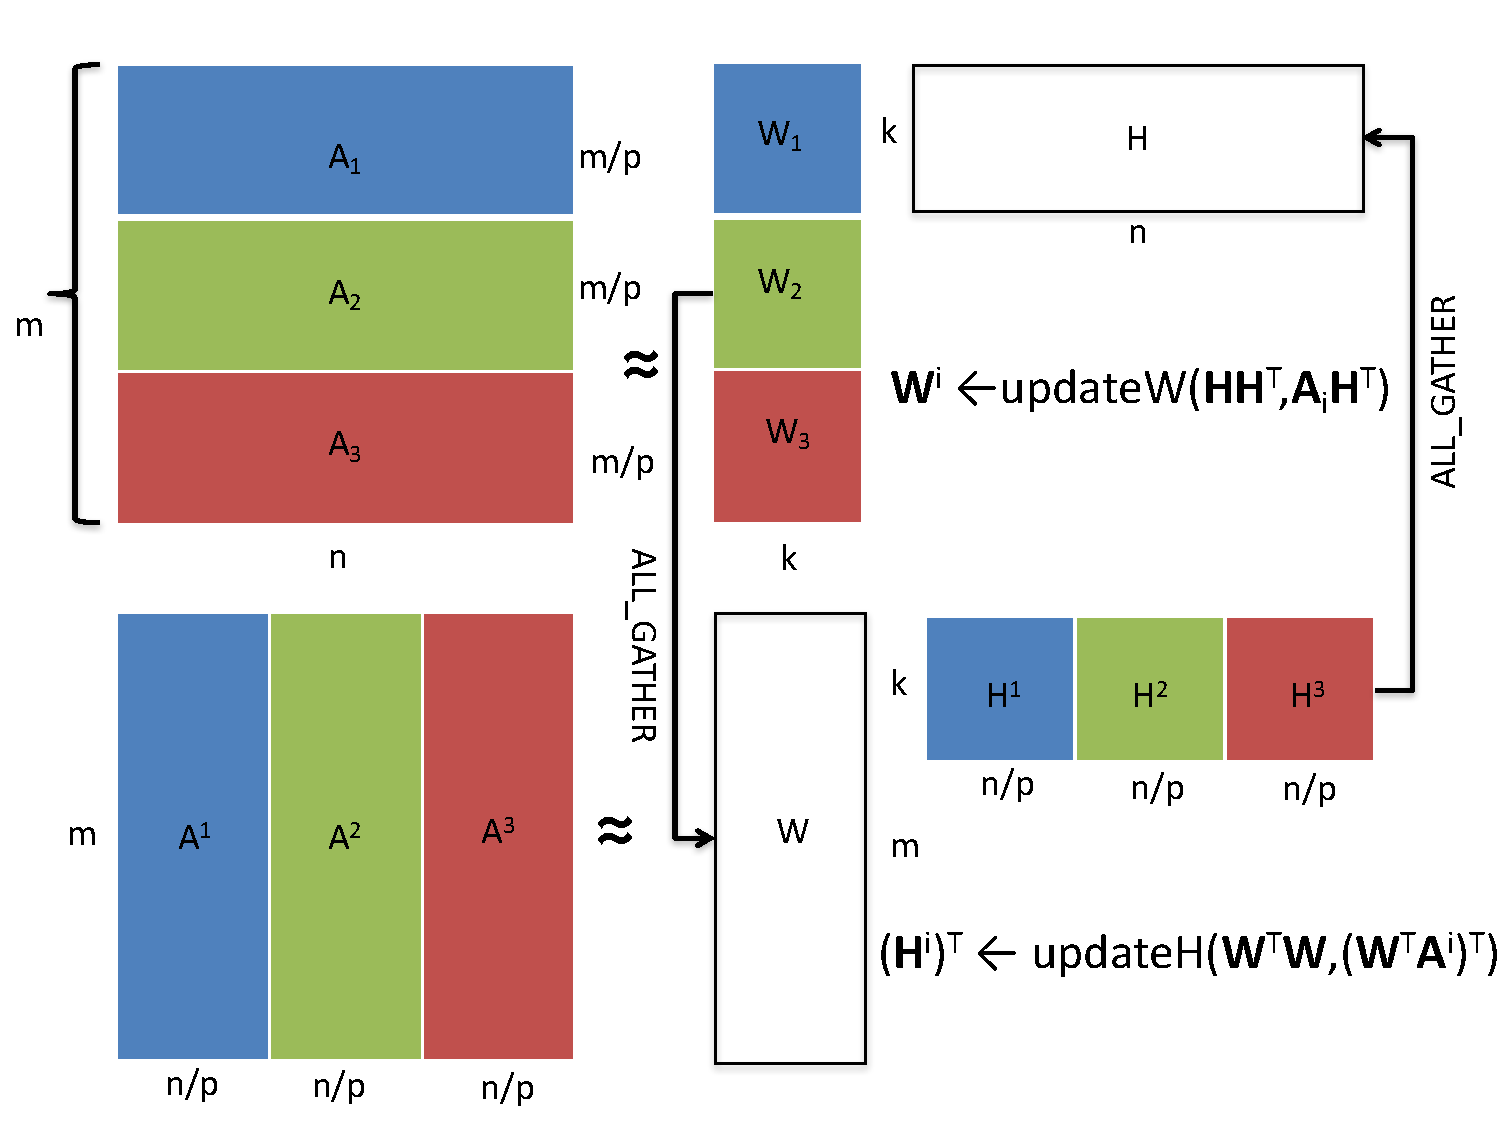
\includegraphics[height=2.5in, width=\columnwidth]{fig/anlsbpp.pdf}
\caption{\NaiveAlg. Both rows and columns of $A$ are 1D distributed.  The algorithm works by (all-)gathering the entire fixed factor matrix to each processor and then performing the Local Update Computations to update the variable factor matrix.} 
\label{fig:naive}
\end{figure}

\renewcommand{\arraystretch}{1.25}
\newcommand{\smallerfont}{\scriptsize}
\begin{table*}[t!]
\begin{center}
\begin{tabular}{|c|c|c|c|c|}
\hline
\textbf{Algorithm} & \textbf{Flops} & \textbf{Words} & \textbf{Messages} & \textbf{Memory}  \\ \hline
\smallerfont \NaiveAlg & \smallerfont $4\frac{mnk}{p}+(m{+}n)k^2+F\lt(\frac mp,\frac np,k\rt)$ & \smallerfont $O((m+n)k)$ & \smallerfont $O(\log p)^*$ & \smallerfont $O\lt(\frac{mn}{p}+(m{+}n)k\rt)$ \\ \hline
\smallerfont \ParNMF\ ($m/p \geq n$) & \smallerfont $4\frac{mnk}{p}+\frac{(m+n)k^2}{p} + F\lt(\frac mp,\frac np,k\rt)$ & \smallerfont $O(nk)$ & \smallerfont $O(\log p)^*$ & \smallerfont $O\lt(\frac{mn}{p}+\frac{mk}{p}+nk\rt)$ \\ \hline
\smallerfont \ParNMF\ ($m/p < n$) & \smallerfont $4\frac{mnk}{p}+\frac{(m+n)k^2}{p}+F\lt(\frac mp,\frac np,k\rt)$ & \smallerfont $O\lt( \sqrt{\frac{mnk^2}{p}}\rt)$ & \smallerfont $O(\log p)^*$ & \smallerfont $O\lt(\frac{mn}{p}+\sqrt{\frac{mnk^2}{p}}\rt)$ \\ \hline
\smallerfont Lower Bound & $-$ & \smallerfont $\Omega\lt(\min\lt\{\sqrt{\frac{mnk^2}{p}},nk\rt\}\rt)$ & \smallerfont $\Omega(\log p)$ & \smallerfont $\frac{mn}{p}+\frac{(m+n)k}{p}$ \\ \hline
\end{tabular}
\normalsize
\end{center}
\caption{Leading order algorithmic costs for \NaiveAlg{} and \ParNMF{} (per iteration).  Note that the computation and memory costs assume the data matrix $\AA$ is dense, but the communication costs (words and messages) apply to both dense and sparse cases.
The function $F(\cdot)$ denotes the number of flops required for the particular NMF algorithm's Local Update Computation, aside from the matrix multiplications common across AU-NMF algorithms. 
Note that $F(m,n,k)$ is proportional to $m+n$ and not $mn$, so the term in the table scales linearly with $p$ (and not $p^2$) for all \LUC. \\
$^*$The stated latency cost assumes no communication is required in \LUC; \HALS\ requires $k\log p$ messages for normalization steps.}
\label{tab:costs}
\end{table*}%

Algorithm \ref{alg:naive} and Figure \ref{fig:naive} present a straightforward approach to parallelizing the independent subproblems.
Let us divide $\WW$ into row blocks $\WW_1, \ldots, \WW_p$ and $\HH$ into column blocks $\HH^1, \ldots, \HH^p$. 
We then double-partition the data matrix $\AA$ accordingly into row blocks $\AA_{1}, \ldots, \AA_p$ and column blocks $\AA^1, \ldots, \AA^p$ so that processor $i$ owns both $\AA_i$ and $\AA^i$ (see Figure \ref{fig:naive}).
With these partitions of the data and the variables, one can implement any AU-NMF algorithm in parallel, with only one communication step for each solve.

We summarize the algorithmic costs of Algorithm \ref{alg:naive} (derived in the following subsections) in Table \ref{tab:costs}.
This naive algorithm \cite{Fairbanks2015} has three main drawbacks: (1) it requires storing two copies of the data matrix (one in row distribution and one in column distribution) and both full factor matrices locally, (2) it does not parallelize the computation of $\HH\HH^T$ and $\WW^T\WW$ (each processor computes it redundantly), and (3) as we will see in Section \ref{sec:parNMF}, it communicates more data than necessary.

\subsubsection{Computation Cost}

The computation cost of Algorithm \ref{alg:naive} depends on the particular NMF algorithm used.
Thus, the computation at line \ref{line:naive:computeW} consists of computing $\AA_i\HH^T$, $\HH\HH^T$, and performing the algorithm-specific Local Update Computations for $m/p$ rows of $\WW$.
Likewise, the computation at line \ref{line:naive:computeH} consists of computing $\WW^T\AA^i$, $\WW^T\WW$, and performing the Local Update Computations for $n/p$ columns of $\HH$.
In the dense case, this amounts to $4mnk/p+(m+n)k^2+F(m/p,n/p,k)$ flops. 
Note that the first term has a constant 4 to account for both $\WW^T\AA$ and $\AA\HH^T$ and that the second term has a constant factor of 1 instead of 2 because the Gram computations ($\HH \HH^T$ and $\WW^T \WW$) exploit symmetry of the output matrix.
In the sparse case, processor $i$ performs $2(\nnz(\AA_i)+\nnz(\AA^i))k$ flops to compute $\AA^i\HH^T$ and $\WW^T\AA_i$ instead of $4mnk/p$. 

\subsubsection{Communication Cost}

The size of $\WW$ is $mk$ words, and the size of $\HH$ is $nk$ words.
Thus, the communication cost of the all-gathers at lines \ref{line:naive:allgatherH} and \ref{line:naive:allgatherW}, based on the expression given in Section \ref{sec:collectives} is $\alpha\cdot 2\log p + \beta\cdot (m+n)k$.

\subsubsection{Memory Requirements} \label{sec:memory}

The local memory requirement includes storing each processor's part of matrices $\AA$, $\WW$, and $\HH$.
In the case of dense $\AA$, this is $2mn/p+(m+n)k/p$ words, as $\AA$ is stored twice; in the sparse case, processor $i$ requires $\nnz(\AA_i)+\nnz(\AA^i)$ words for the input matrix and $(m+n)k/p$ words for the output factor matrices.
Local memory is also required for storing temporary matrices $\WW$ and $\HH$ of size $(m+n)k$ words.


\subsection{\ParNMF}
\label{sec:parNMF}

We present our proposed algorithm, \ParNMF, as Algorithm \ref{alg:2D} and Figure \ref{fig:2D-Algorithm}. 
The main ideas of the algorithm are to (1) exploit the independence of Local Update Computations for rows of $\WW$ and columns of $\HH$ and (2) use communication-optimal matrix multiplication algorithms to set up the Local Update Computations.
The naive approach (Algorithm \ref{alg:naive}) shares the first property, by parallelizing over rows of $\WW$ and columns of $\HH$, but it uses parallel matrix multiplication algorithms that communicate more data than necessary.
The central intuition for communication-efficient parallel algorithms for computing $\HH\HH^T$, $\AA\HH^T$, $\WW^T\WW$, and $\WW^T\AA$ comes from a classification proposed by Demmel et al. \cite{DE+13}.
They consider three cases, depending on the relative sizes of the dimensions of the matrices and the number of processors; the four multiplies for NMF fall into either the ``one large dimension'' or ``two large dimensions" cases.
\ParNMF\ uses a careful data distribution in order to use a communication-optimal algorithm for each of the matrix multiplications, while at the same time exploiting the parallelism in the \LUC.

The algorithm uses a 2D distribution of the data matrix $\AA$ across a $p_r \times p_c$ grid of processors (with $p=p_rp_c$), as shown in Figure \ref{fig:2D-distribution}.
As we derive in the subsequent subsections, Algorithm \ref{alg:2D} performs an alternating method in parallel with a per-iteration bandwidth cost of $O\lt(\min\lt\{\sqrt{mnk^2/p},nk\rt\}\rt)$ words, latency cost of $O(\log p)$ messages, and load-balanced computation (up to the sparsity pattern of $\AA$ and convergence rates of local BPP computations). Figure \ref{fig:2D-Algorithm}, illustrates determining $\HH$ given $\WW$ with $pr=3$ and $pc=2$. 

The main improvement of \ParNMF\ over \Naive\ involves the computation of $\AA\HH^T$ and $\WW^T\AA$.
By using a 2D distribution of the data matrix, no processor needs access to \emph{all} of one factor matrix, as in the case of \Naive, where each processor must access either all $m$ rows of $\WW$ or all $n$ columns of $\HH$.
Instead, with \ParNMF, each processor must access only $m/p_r$ of the rows of $\WW$ and $n/p_c$ of the columns of $\HH$, so the number of rows decreases as $p$ increases.
This implies the communication cost is reduced, as verified empirically in Figure \ref{fig:procsweep} (the extreme cases correspond to 1D distributions).

To minimize the communication cost and local memory requirements, in the typical case $p_r$ and $p_c$ are chosen so that $m/p_r\approx n/p_c\approx \sqrt{mn/p}$, in which case the bandwidth cost is $O\lt(\sqrt{mnk^2/p}\rt)$.
If the matrix is very tall and skinny, i.e., $m/p>n$, then we choose $p_r=p$ and $p_c=1$.
In this case, the distribution of the data matrix is 1D, and the bandwidth cost is $O(nk)$ words.

The matrix distributions for Algorithm \ref{alg:2D} are given in Figure \ref{fig:2D-distribution}; we use a 2D distribution of $\AA$ and 1D distributions of $\WW$ and $\HH$.
Recall from Table \ref{tab:notation} that $\M{M}_i$ and $\M{M}^i$  denote row and column blocks of $\M{M}$, respectively.
Thus, the notation $(\WW_i)_j$ denotes the $j$th row block within the $i$th row block of $\WW$.
Lines \ref{line:2DsyrkH}--\ref{line:2DcompW} compute $\WW$ for a fixed $\HH$, and lines \ref{line:2DsyrkW}--\ref{line:2DcompH} compute $\HH$ for a fixed $\WW$; note that the computations and communication patterns for the two alternating iterations are analogous.

In the rest of this section, we derive the per-iteration computation and communication costs, as well as the local memory requirements.
We also argue the communication-optimality of the algorithm in the dense case.
Table \ref{tab:costs} summarizes the results of this section and compares them to \NaiveAlg.

\begin{algorithm}[t!]
\caption{$[\WW,\HH] = \text{\ParNMF}(\AA,k)$}
\label{alg:2D}
\begin{algorithmic}[1]
\small
\Require $\AA$ is an $m\times n$ matrix distributed across a $p_r\times p_c$ grid of processors, $k$ is rank of approximation
\Require Local matrices: $\AA_{ij}$ is $m/p_r\times n/p_c$, $\WW_i$ is $m/p_r\times k$, $(\WW_i)_j$ is $m/p\times k$, $\HH_j$ is $k\times n/p_c$, and $(\HH_j)_i$ is $k\times n/p$
\State $p_{ij}$ initializes $(\HH_j)_i$
\While{stopping criteria not satisfied}
	\Statex \quad\; \textbf{/* Compute $\WW$ given $\HH$ */} 
	\State $p_{ij}$ computes $\M{U}_{ij}=(\HH_j)_i{(\HH_j)_i}^T$
		\label{line:2DsyrkH}
	\State compute $\HH\HH^T {=} \sum_{i,j} \M{U}_{ij}$ using all-reduce across all procs
		\label{line:2Dall-reduceH}
		\Comment{$\HH\HH^T$ is $k\times k$ and symmetric}
	\State $p_{ij}$ collects $\HH_j$ using all-gather across proc columns
		\label{line:2Dall-gatherH}
	\State $p_{ij}$ computes $\M{V}_{ij}=\AA_{ij}\HH_j^T$
		\label{line:2DNEW}
		\Comment{$\M{V}_{ij}$ is $m/p_r \times k$}
	\State compute $(\AA\HH^T)_i {=} \sum_j \M{V}_{ij}$ using reduce-scatter across proc row to achieve row-wise distribution of $(\AA\HH^T)_i$
		\Comment{$p_{ij}$ owns $m/p\times k$ submatrix $((\AA\HH^T)_i)_j$}
		\label{line:2Dreduce-scatterAHT}
		%\Statex \Comment{Use Equation \eqref{eqn:muupdate},\eqref{eqn:halsupdate} for \MU\ and \HALS\ respectively. ANLS/BPP will implement the SolveBPP function \ref{sec:BPP}.} 	
	\State $p_{ij}$ computes $(\WW_i)_j \gets$ UpdateW $(\HH\HH^T,((\AA\HH^T)_i)_j)$
		\label{line:2DcompW}
	\Statex \quad\; \textbf{/* Compute $\HH$ given $\WW$ */}
	\State $p_{ij}$ computes $\M{X}_{ij}={(\WW_i)_j}^T(\WW_i)_j$
		\label{line:2DsyrkW}
	\State compute $\WW^T\WW {=} \sum_{i,j} \M{X}_{ij}$ using all-reduce across all procs
		\label{line:2Dall-reduceW}
		\Comment{$\WW^T\WW$ is $k\times k$ and symmetric}
	\State $p_{ij}$ collects $\WW_i$ using all-gather across proc rows
		\label{line:2Dall-gatherW}
	\State $p_{ij}$ computes $\M{Y}_{ij}={\WW_i}^T\AA_{ij}$
		\label{line:2DNEH}
		\Comment{$\M{Y}_{ij}$ is $k\times n/p_c$}
	\State compute $(\WW^T\AA)^j = \sum_i \M{Y}_{ij}$ using reduce-scatter across proc columns to achieve column-wise distribution of $(\WW^T\AA)^j$
		\Comment{$p_{ij}$ owns $k\times n/p$ submatrix $((\WW^T\AA)^j)^i$}
		\label{line:2Dreduce-scatterWTA}
		%\Statex \Comment{Use Equation \eqref{eqn:muupdate},\eqref{eqn:halsupdate} for \MU\ and \HALS\ respectively. ANLS/BPP will implement the SolveBPP function \ref{sec:BPP}.}
	\State $p_{ij}$ computes $((\HH^j)^i)^T \gets$ UpdateH $(\WW^T\WW,(((\WW^T\AA)^j)^i)^T)$
		\label{line:2DcompH}
\EndWhile
\Ensure $\displaystyle \WW, \HH \approx \Argmin{\M{\tilde W} \geq 0, \M{\tilde H} \geq 0} \|\AA- \M{\tilde W} \M{\tilde H}\|$
\Ensure $\WW$ is an $m\times k$ matrix distributed row-wise across processors, $\HH$ is a $k\times n$ matrix distributed column-wise across processors
\normalsize
\end{algorithmic}
\end{algorithm}

\begin{figure}[t!]
\centering
\begin{subfigure}[b]{0.3\columnwidth}
\centering
\scalebox{.7}{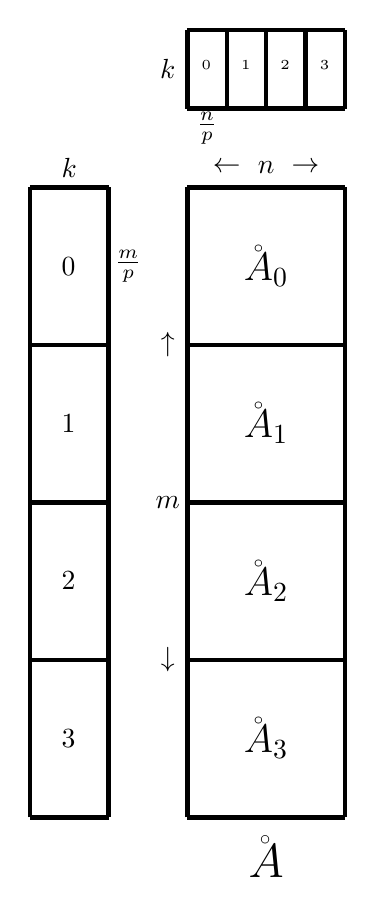
\begin{tikzpicture}

%% draw matrix distributions with scaled grids
% A
\draw[xscale=2,yscale=2,ultra thick] (0,0) grid (1,4);
% W
\draw[yscale=2,ultra thick] (-2,0) grid (-1,4);
% H
\draw[xscale=1/2,ultra thick] (0,9) grid (4,10);

%% add (sub)matrix names 
% A
\node[draw=none] at (1,-0.5) {\LARGE $\AA$};
\node[draw=none] at (1,7) {\Large $\AA_0$};
\node[draw=none] at (1,5) {\Large $\AA_1$};
\node[draw=none] at (1,3) {\Large $\AA_2$};
\node[draw=none] at (1,1) {\Large $\AA_3$};
% W
\node[draw=none] at (-1.5,-0.5) {\LARGE $\WW$};
\node[draw=none] at (-1.5,7) {\Large $\WW_0$};
\node[draw=none] at (-1.5,5) {\Large $\WW_1$};
\node[draw=none] at (-1.5,3) {\Large $\WW_2$};
\node[draw=none] at (-1.5,1) {\Large $\WW_3$};
% H
\node[draw=none] at (-1,9.5) {\LARGE $\HH$};
\node[draw=none] at (0.25,9.5) {\scriptsize $\HH^0$};
\node[draw=none] at (0.75,9.5) {\scriptsize $\HH^1$};
\node[draw=none] at (1.25,9.5) {\scriptsize $\HH^2$};
\node[draw=none] at (1.75,9.5) {\scriptsize $\HH^3$};

% label vertical dimensions
\node[draw=none] at (-0.25,9.5) {$k$};
\node[draw=none] at (-0.25,4) {$m$};
\node[draw=none] at (-0.25,6) {$\uparrow$};
\node[draw=none] at (-0.25,2) {$\downarrow$};
\node[draw=none] at (-0.75,7) {$\frac{m}{p}$};
% label horizontal dimensions
\node[draw=none] at (-1.5,8.25) {$k$};
\node[draw=none] at (1,8.25) {$n$};
\node[draw=none] at (0.5,8.25) {$\leftarrow$};
\node[draw=none] at (1.5,8.25) {$\rightarrow$};
\node[draw=none] at (0.25,8.75) {$\frac{n}{p}$};

\end{tikzpicture}
}
%\subcaption{1D Distribution with $p=p_r=4$ and $p_c=1$.}
\label{1D}
\end{subfigure} 
~
\begin{subfigure}[b]{0.6\columnwidth}
\centering
\scalebox{.75}{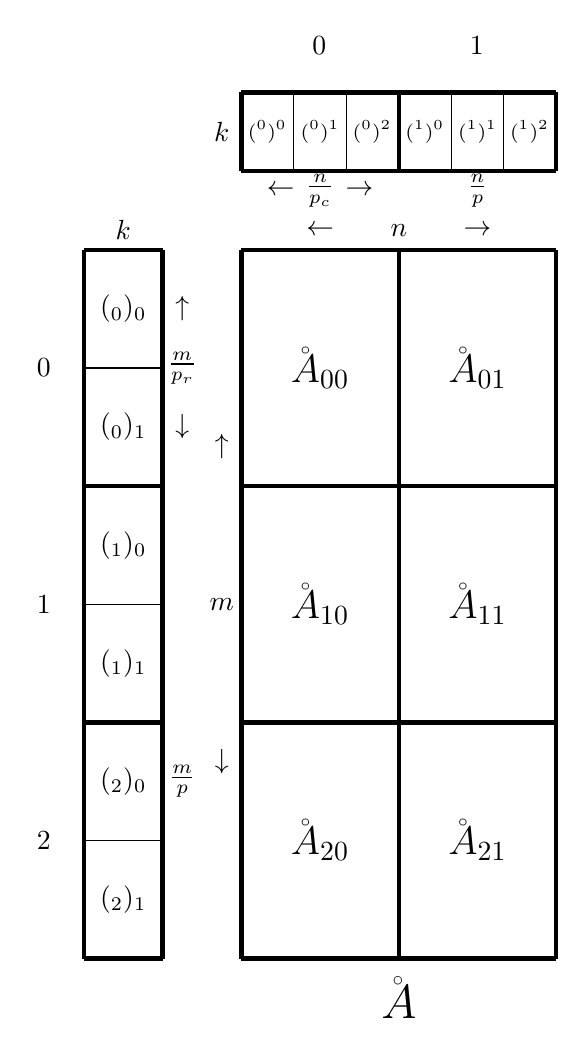
\begin{tikzpicture}

%% draw matrix distributions with scaled grids
% A
\draw[xscale=2,yscale=3,ultra thick] (0,0) grid (2,3);
% W
\draw[yscale=3/2] (-2,0) grid (-1,6);
\draw[yscale=3,ultra thick] (-2,0) grid (-1,3);
% H
\draw[xscale=2/3] (0,10) grid (6,11);
\draw[xscale=2,ultra thick] (0,10) grid (2,11);

%% add (sub)matrix names 
% A
\node[draw=none] at (2,-0.5) {\LARGE $\AA$};
\node[draw=none] at (1,7.5) {\Large $\AA_{00}$};
\node[draw=none] at (1,4.5) {\Large $\AA_{10}$};
\node[draw=none] at (1,1.5) {\Large $\AA_{20}$};
\node[draw=none] at (3,7.5) {\Large $\AA_{01}$};
\node[draw=none] at (3,4.5) {\Large $\AA_{11}$};
\node[draw=none] at (3,1.5) {\Large $\AA_{21}$};
% W
\node[draw=none] at (-1.5,-0.5) {\LARGE $\WW$};
\node[draw=none] at (-2.5,7.5) {\Large $\WW_0$};
\node[draw=none] at (-2.5,4.5) {\Large $\WW_1$};
\node[draw=none] at (-2.5,1.5) {\Large $\WW_2$};
\node[draw=none] at (-1.5,8.25) {$(\WW_0)_0$};
\node[draw=none] at (-1.5,6.75) {$(\WW_0)_1$};
\node[draw=none] at (-1.5,5.25) {$(\WW_1)_0$};
\node[draw=none] at (-1.5,3.75) {$(\WW_1)_1$};
\node[draw=none] at (-1.5,2.25) {$(\WW_2)_0$};
\node[draw=none] at (-1.5,0.75) {$(\WW_2)_1$};
% H
\node[draw=none] at (-1,10.5) {\LARGE $\HH$};
\node[draw=none] at (1,11.5) {\Large $\HH^0$};
\node[draw=none] at (3,11.5) {\Large $\HH^1$};
\node[draw=none] at (.33,10.5) {\scriptsize $(\HH^0)^0$};
\node[draw=none] at (1,10.5) {\scriptsize $(\HH^0)^1$};
\node[draw=none] at (1.66,10.5) {\scriptsize $(\HH^0)^2$};
\node[draw=none] at (2.33,10.5) {\scriptsize $(\HH^1)^0$};
\node[draw=none] at (3,10.5) {\scriptsize $(\HH^1)^1$};
\node[draw=none] at (3.66,10.5) {\scriptsize $(\HH^1)^2$};

% label vertical dimensions
\node[draw=none] at (-0.25,10.5) {$k$};
\node[draw=none] at (-0.25,4.5) {$m$};
\node[draw=none] at (-0.25,6.5) {$\uparrow$};
\node[draw=none] at (-0.25,2.5) {$\downarrow$};
\node[draw=none] at (-0.75,7.5) {$\frac{m}{p_r}$};
\node[draw=none] at (-0.75,8.25) {$\uparrow$};
\node[draw=none] at (-0.75,6.75) {$\downarrow$};
\node[draw=none] at (-0.75,2.25) {$\frac{m}{p}$};
% label horizontal dimensions
\node[draw=none] at (-1.5,9.25) {$k$};
\node[draw=none] at (2,9.25) {$n$};
\node[draw=none] at (1,9.25) {$\leftarrow$};
\node[draw=none] at (3,9.25) {$\rightarrow$};
\node[draw=none] at (1,9.75) {$\frac{n}{p_c}$};
\node[draw=none] at (0.5,9.75) {$\leftarrow$};
\node[draw=none] at (1.5,9.75) {$\rightarrow$};
\node[draw=none] at (3,9.75) {$\frac{n}{p}$};

\end{tikzpicture}}
%\subcaption{2D Distribution with $p_r=3$ and $p_c=2$.}
\label{2D}
\end{subfigure}
\caption{Data distributions for \ParNMF. 1D Distribution on left with $p=p_r=4$ and $p_c=1$. 2D Distribution on right with $p_r=3$ and $p_c=2$
Note that for the 2D distribution, $\AA_{ij}$ is $m/p_r \times m/p_c$, $\WW_i$ is $m/p_r \times k$, $(\WW_i)_j$ is $m/p\times k$, $\HH_j$ is $k\times n/p_c$, and $(\HH^j)^i$ is $k\times n/p$.}
\label{fig:2D-distribution}
\end{figure}
~
\begin{figure*}[t!]
\centering
\includegraphics[width=0.8\textwidth, height=3in]{fig/mm2D.pdf}
\caption{Parallel matrix multiplications within \ParNMF\ for finding $\HH$ given $\WW$, with $p_r=3$ and $p_c=2$.  The computation of $\WW^T\WW$ appears on the far left; the rest of the figure depicts computation of $\WW^T\AA$.}
\label{fig:2D-Algorithm}
\end{figure*}


\subsubsection{Computation Cost}

Local matrix computations occur at lines \ref{line:2DsyrkH}, \ref{line:2DNEW}, \ref{line:2DsyrkW}, and \ref{line:2DNEH}.
In the case that $\AA$ is dense, each processor performs 
$$\frac np k^2+2\frac{m}{p_r}\frac{n}{p_c}k+\frac mp k^2+2\frac{m}{p_r}\frac{n}{p_c}k=4\frac{mnk}{p}+\frac{(m+n)k^2}{p}$$
flops. 
Recall that the second term on the right hand side has a constant factor of 1 instead of 2 because the local Gram computations (lines \ref{line:2DsyrkH} and \ref{line:2DsyrkW}) exploit symmetry.
In the case that $\AA$ is sparse, processor $(i,j)$ performs $(m+n)k^2/p$ flops in computing $\M{U}_{ij}$ and $\M{X}_{ij}$, and $4\nnz(\AA_{ij})k$ flops in computing $\M{V}_{ij}$ and $\M{Y}_{ij}$.
Local update computations occur at lines \ref{line:2DcompW} and \ref{line:2DcompH}.
In each case, the symmetric positive semi-definite matrix is $k\times k$ and the number of columns/rows of length $k$ to be computed are $m/p$ and $n/p$, respectively.
These costs together are given by $F(m/p,n/p,k)$.
There are computation costs associated with the all-reduce and reduce-scatter collectives (see Section \ref{sec:collectives}), both those contribute only to lower order terms: $O(k^2+mk/p_r+nk/p_c)$.

\subsubsection{Communication Cost}
\label{sec:alg:comm}

Communication occurs during six collective operations (lines \ref{line:2Dall-reduceH}, \ref{line:2Dall-gatherH}, \ref{line:2Dreduce-scatterAHT}, \ref{line:2Dall-reduceW}, \ref{line:2Dall-gatherW}, and \ref{line:2Dreduce-scatterWTA}).
We use the cost expressions presented in Section \ref{sec:collectives} for these collectives.
The communication cost of the all-reduces (lines \ref{line:2Dall-reduceH} and \ref{line:2Dall-reduceW}) is $\alpha \cdot 4\log p+\beta \cdot 2k^2$; 
the cost of the two all-gathers (lines \ref{line:2Dall-gatherH} and \ref{line:2Dall-gatherW}) is $\alpha \cdot \log p + \beta \cdot \lt( (p_r{-}1)nk/p + (p_c{-}1)mk/p\rt)$; and
the cost of the two reduce-scatters (lines \ref{line:2Dreduce-scatterAHT} and  \ref{line:2Dreduce-scatterWTA}) is $\alpha \cdot \log p + \beta \cdot \lt( (p_c{-}1)mk/p + (p_r{-}1)nk/p\rt)$.

We note that \LUC\ may introduce significant communication cost, depending on the NMF algorithm used.
The normalization of columns of $\WW$ within \HALS, for example, introduces an extra $k\log p$ latency cost.
We will ignore such costs in our general analysis.

In the case that $m/p<n$, we choose $p_r=\sqrt{mp/n} >1$ and $p_c=\sqrt{np/m}>1$, and these communication costs simplify to $\alpha \cdot O(\log p) + \beta \cdot O(mk/p_r+nk/p_c+k^2) = \alpha \cdot O(\log p) + \beta \cdot O(\sqrt{mnk^2/p}+k^2)$.
In the case that $m/p\geq n$, we choose $p_c=1$, and the costs simplify to $\alpha \cdot O(\log p) + \beta \cdot O(nk)$.

\ignore{
Thus, the total cost per iteration is
$$\gamma \cdot O\lt( \frac{mnk}{p} + C_\text{BPP}\lt(k,\frac{m+n}{p}\rt) \rt) + \beta \cdot O\lt(\frac{mk}{p_r}+\frac{nk}{p_c}+k^2\rt) + \alpha \cdot O(\log p).$$
In order to minimize the bandwidth cost of the algorithm, we choose $p_r=\sqrt{mp/n}$ and $p_c=\sqrt{np/m}$; this yields a per-iteration cost of 
$$\gamma \cdot O\lt( \frac{mnk}{p} + C_\text{BPP}\lt(k,\frac{m+n}{p}\rt) \rt) + \beta \cdot O\lt(\sqrt{\frac{mnk^2}{p}}+k^2\rt) + \alpha \cdot O(\log p).$$
We note that these choices of $p_r$ and $p_c$ are well defined assuming $m/p<n$ and $n/p<m$; if one of these assumptions is not satisfied we resort to Algorithm \ref{alg:1D}.
}

\subsubsection{Memory Requirements}
\label{sec:new_memory}

The local memory requirement includes storing each processor's part of matrices $\AA$, $\WW$, and $\HH$.
In the case of dense $\AA$, this is $mn/p+(m+n)k/p$ words; in the sparse case, processor $(i,j)$ requires $\nnz(\AA_{ij})$ words for the input matrix and $(m+n)k/p$ words for the output factor matrices.
Local memory is also required for storing temporary matrices $\WW_j$, $\HH_i$, $\M{V}_{ij}$, and $\M{Y}_{ij}$, of size $2mk/p_r+2nk/p_c$ words.

In the dense case, assuming $k<n/p_c$ and $k<m/p_r$, the local memory requirement is no more than a constant times the size of the original data.
For the optimal choices of $p_r$ and $p_c$, this assumption simplifies to $k<\max\lt\{\sqrt{mn/p},m/p\rt\}$. 
Note that the second argument of the max applies when the optimal distribution is 1D ($p_r=p$).

We note that if the temporary memory requirements become prohibitive, the computation of $((\AA \HH^T)_i)_j$ and $((\WW^T\AA)_j)_i$ via all-gathers and reduce-scatters can be blocked, decreasing the local memory requirements at the expense of greater latency costs.
When $\AA$ is sparse and $k$ is large enough, the memory footprint of the factor matrices can be larger than the input matrix.
In this case, the extra temporary memory requirements can become prohibitive; we observed this for a sparse data set with very large dimensions (see Section \ref{sec:webbase-2001}).
We leave the implementation of the blocked algorithm to future work.


\subsubsection{Communication Optimality}

In the case that $\AA$ is dense, Algorithm \ref{alg:2D} provably minimizes communication costs.
Theorem \ref{thm:LB} establishes the bandwidth cost lower bound for any algorithm that computes $\WW^T\AA$ or $\AA\HH^T$ each iteration.
A latency lower bound of $\Omega(\log p)$ exists in our communication model for any algorithm that aggregates global information \cite{CH+07}.
For NMF, this global aggregation is necessary in each iteration, for example, in order to compute residual error in the case that $\AA$ is distributed across all $p$ processors, because all processors have data that must be accumulated into the global error.
Based on the costs derived above, \ParNMF\ is communication optimal under the assumption $k<\sqrt{mn/p}$, matching these lower bounds to within constant factors.

\begin{theorem}[\cite{DE+13}]
\label{thm:LB}
Let $\AA \in \Rn{m \times n}$, $\WW \in \Rn{m \times k}$, and $\HH \in \Rn{k \times n}$ be dense matrices, with $k<n\leq m$.  If $k < \sqrt{mn/p}$, then any distributed-memory parallel algorithm on $p$ processors that load balances the matrix distributions and computes $\WW^T \AA$ and/or $\AA \HH^T$ must communicate at least $\Omega(\min\{\sqrt{mnk^2/p},nk\})$ words along its critical path.
\end{theorem}
\begin{proof}
The proof follows directly from \cite[Section II.B]{DE+13}.
Each matrix multiplication $\WW^T \AA$ and $\AA \HH^T$ has dimensions $k<n\leq m$, so the assumption $k<\sqrt{mn/p}$ ensures that neither multiplication has ``3 large dimensions.''
Thus, the communication lower bound is either $\Omega(\sqrt{mnk^2/p})$ in the case of $p>m/n$ (or ``2 large dimensions''), or $\Omega(nk)$, in the case of $p<m/n$ (or ``1 large dimension'').
If $p<m/n$, then $nk<\sqrt{mnk^2/p}$, so the lower bound can be written as $\Omega(\min\{\sqrt{mnk^2/p},nk\})$.
\end{proof}

We note that the communication costs of Algorithm \ref{alg:2D} are the same for dense and sparse data matrices (the data matrix itself is never communicated).
In the case that $\AA$ is sparse, this communication lower bound does not necessarily apply, as the required data movement depends on the sparsity pattern of $\AA$.
Thus, we cannot make claims of optimality in the sparse case (for general $\AA$).
The communication lower bounds for $\WW^T \AA$ and/or $\AA \HH^T$ (where $\AA$ is sparse) can be expressed in terms of hypergraphs that encode the sparsity structure of $\AA$ \cite{BDKS15}.
Indeed, hypergraph partitioners have been used to reduce communication and achieve load balance for a similar problem: computing a low-rank representation of a sparse tensor (without non-negativity constraints on the factors) \cite{KU15}.

